\chapter{Background \& Related Work}
\label{ch:Background}

\newcommand{\ea}[2]{#1 \text{et al.} #2}


%50-100 pages
%Introduction
%Hardware and such narrow down target users - potential users
%Adults make not sense using touching learning ()
%Adult vs child group comparison - maybe change some papers

%Not always refers to articles, but also to commercial products
%Create own citation based on minimum inforamation
%Summarise applications which are out there

%Is there a gold standard for braille learning for sighted people

%Haptic braille learning paper

%Special experts could use the application
%Let expert try out final report
%Let try out potential users (specify the potential users) —> sight adults \ exclude non adult literature also in design 
%Backward chain of papers - commonly used method.

%Intro, discussion 10
%30 methods
%30 related work

\section{Passive learning}
Learning is often perceived as an active and purposive process; however, this is not always the case. In addition to active learning, there exists a form of passive learning, which stands in contrast to the active approach. Passive learning is often described as being \enquote{caught rather than taught} \cite{krugman1970passive}, emphasizing its effortless nature. This lack of effort is attributed to the absence of resistance, meaning that neither motivation nor interest is necessary for the acquisition of this type of knowledge \cite{Zukin1984}.
Furthermore, passive learning has been characterized as “typically effortless, responsive to animated stimuli, amenable to artificial aids to relaxation, and marked by an absence of resistance to what is learned” \cite{Huang2008,krugman1970passive}. This suggests that passive learning can occur in environments where learners are exposed to stimuli without actively engaging in the learning process.
Zukin et al. \cite{Zukin1984} demonstrated that exposure to media-rich environments can lead to information being acquired passively. In their study, they examined two groups of subjects who were not initially interested in political information. They found that subjects who were exposed to political content through a media-rich environment were 40\% more likely to acquire the information compared to those living in media-poor environments \cite{zukin1984passive, Huang2008}.
Later research by Huang et al. \cite{Huang2008} extended the concept of passive learning to the acquisition of physical skills. The success of this study contributed to the introduction of the term \gls{phl} \cite{Pescara2019}, which further encapsulates the potential for learning in contexts where active engagement is minimal or absent.
Over the years a significant body of research has been dedicated to the exploration of \gls{phl}. It spanned a wide range of applications, including piano learning \cite{Huang2008, Kohlsdorf2010, Seim2015b, Donchev2021, Fang2023a, Fang2023}, the acquisition of typing skills \cite{Seim2014, Seim2017, Seim2014a, Learning2024}, the learning of Braille \cite{Seim2014a, Learning2024}, Morse code \cite{Seim2016a, Seim2018, Pescara2019}, multi-limb rhythm coordination \cite{Bouwer2011, Holland2010}, skin reading \cite{Luzhnica2016, Luzhnica2018}, and even the effects of \gls{phl} on spinal cord injury (SCI) rehabilitation \cite{Markow2010}.


%-----
\subsection*{Distraction Task}
\begin{table}[!ht]
\centering
\resizebox{\columnwidth}{!}{
\begin{tabular}{|l|l|l|l|l|l|}
    \hline
        \textbf{Paper name} & \textbf{Game} & \textbf{Learning Time} \\ \hline
        \ea{Caulfield}{\cite{Learning2024}} &  Not mentioned & 10 min \\ \hline
        \ea{Fang}{\cite{Fang2023}} &  Gweled  & 30 min \\ \hline
        \ea{Fang}{\cite{Fang2023a}} &  Tetris & 15 min \\ \hline
        \ea{Donchev}{\cite{Donchev2021}} &  Gweled & 20 min \\ \hline
        \ea{Hsu}{\cite{Hsu2021}} & Not mentioned & 30 min \\ \hline
        \ea{Pescara}{\cite{Pescara2019}} & \specialcell{Gweled\\ Open Hexagon} & \specialcell{20 min \\(5 min training/character)} \\ \hline
        \ea{Luzhnica}{\cite{Luzhnica2018}} &  Snake Game & 32 min \\ \hline
        \ea{Seim}{\cite{Seim2018}} &  Fritz & 8 or 16 min \\ \hline
        \ea{Seim}{\cite{Seim2017}} &  Fritz & 15 min \\ \hline
        \ea{Seim}{\cite{Seim2016a}} &  Fritz & 20 min \\ \hline
        \ea{Seim}{\cite{Seim2015b}} &  Fritz & 20 min \\ \hline
        \ea{Seim}{\cite{Seim2014}} & Memory Card Game & 30 min \\ \hline
        \ea{Seim}{\cite{Seim2014a}} & Fritz &  30 min \\ \hline
        \ea{Bouwer}{\cite{Bouwer2011}} &  Reading Comprehension &  30 min \\ \hline
        \ea{Kohlsdorf}{\cite{Kohlsdorf2010}} &  \specialcell{Watching a film\\Playing memory\\Walking a path} & 5 min \\ \hline
        \ea{Huang}{\cite{Huang2010}} & \specialcell{Daily task (pilot study)\\ PSAT/SAT (main study)} & 30 min \\ \hline
        \ea{Pala}{\cite{Vaio6810}} &  Not mentioned & 15-60 min \\ \hline
        \ea{Huang}{\cite{Huang2008}} & \specialcell{Daily task\\ (Reading book/paper, typing at desk)} & 30 min \\ \hline
    \end{tabular}
    
}
\caption{Distraction tasks leveraged in previous literature.}
\label{tab:distraction_tasks}
\end{table}

Apart from the primary challenges of learning new skills or rehabilitation, much of the focus in \gls{phl} research has been on distraction tasks, which are crucial to its main selling point. Distraction tasks are those that can be performed concurrently while the primary learning process takes place, allowing the acquisition of information to occur passively. We compared the distraction tasks used in previous literature, along with the time participants spent learning, and summarized them in \autoref{tab:distraction_tasks}.

In earlier \gls{phl} research, reading comprehension tests \cite{Huang2008, Huang2010, Kohlsdorf2010} were commonly employed as the distraction task. However, this method has largely fallen out of favour. During the development of the \gls{mmt} framework, Kohlsdorf et al. \cite{Kohlsdorf2010} tested three different tasks: watching a film (audio-visual stimulation), playing a memory game (active memory engagement), and walking a designated path (body motion). These tasks were chosen to represent common everyday activities such as relaxing, thinking, and walking.

The results showed no statistically significant difference in the number of \gls{phl} sessions required across the different tasks. However, individual differences emerged, with some participants finding certain tasks more challenging than others. Rhythm retention was slightly better after the memory game condition compared to the film condition, though no condition was significantly better or worse overall. Participants reported similar subjective workloads across all conditions, suggesting that the type of primary task does not significantly impact the effectiveness of \gls{phl} in learning piano sequences. The study concluded that while the type of primary task may influence individual performance, there is no clear evidence that one task is superior to others in enhancing \gls{phl} effectiveness. This suggests that \gls{phl} can be integrated into various everyday activities without being significantly hindered by the nature of the concurrent task.

This was also investigated by \citet{Pescara2019}, who found that the difficulty level of distraction tasks, such as the games Gweled (easy) and Open Hexagon\footnote{Open Hexagon: \url{https://vittorioromeo.info/Downloads/}} (hard), did not significantly influence learning outcomes \cite{Pescara2019}. However, Pescara et al. also noted that participants reported increased fatigue over the course of the study due to the prolonged focus required by these games. This finding suggests that future research should explore alternative distraction tasks that are engaging enough to divert attention from \gls{phl}, yet unlikely to induce fatigue during extended periods—a challenge that remains difficult to address.

More recent studies have shifted their focus to other tasks, such as playing the game 'Fritz'\footnote{Fritz!: \url{www.gamesgames.com/game/fitz.}}, which has become the most frequently used alternative, appearing in five studies, followed by the game 'Gweled,'\footnote{Gweled: \url{https://gweled.org}} which has been utilized in three studies. \autoref{tab:distraction_tasks} provides an overview of the games used as distraction tasks in previous literature.


\subsection*{PHL Duration}
Another crucial factor is the duration of the distraction task and the period during which passive learning occurs, as this may directly influence the effectiveness of the \gls{phl} process. As shown in \autoref{tab:distraction_tasks}, most studies employ a standard learning period of 30 minutes before subjects undergo further testing or evaluation. Close behind, several studies opt for a slightly shorter 20-minute learning period. However, there is significant variability in session lengths, ranging from as brief as 5 minutes to as long as 60 minutes, indicating no clear consensus on the optimal duration. To explore this further, Seim's study \cite{Seim2018} highlighted the benefits of extended learning time. The study demonstrated a notable improvement in learning Morse code between 8-minute and 16-minute exposure conditions, suggesting that longer exposure periods may be more advantageous.

\subsection*{Overlearning}
Another aspect closely tied to learning duration is the concept of overlearning. Overlearning refers to the deliberate overtraining of an already learned task, aiming to achieve error-free performance \cite{Krueger1929}. Numerous psychological studies have examined its effects, particularly on retention \cite{Krueger1929, Driskell1992}. While overlearning can enhance retention, it may also have adverse effects, such as degrading performance, as demonstrated by Langer et al. \cite{Langer1979}.

In the context of \gls{phl}, Donchev et al. \cite{Donchev2021} deliberately avoided overlearning, citing its unpredictable effects on long-term retention and the potential for distorted results. To mitigate this, they halted the learning session once participants achieved an accuracy of 90% or higher.

However, not all studies have avoided overlearning. For example, Seim et al. \cite{Seim2016, Seim2014a} included overlearning in their experimental design. In their full alphabet study \cite{Seim2014a}, they specifically investigated its effects. Conversely, in another study \cite{Seim2015}, they avoided overlearning to prevent ceiling effects on shorter phrases. This suggests that the decision to include overlearning in some studies was likely a deliberate choice tailored to the research objectives.

\subsection*{Chunking}
When learning information, it is often presented piece by piece. This is called \enquote{chunking} and it is a critical concept in cognitive science, especially in memory and learning processes. It involves breaking large pieces of information into smaller, more manageable units to enhance retention. \ea{Miller}{\cite{miller1956}} first observed that the average person can hold about seven items in working memory, and that chunking helps organize information into meaningful patterns. \ea{Laird}{\cite{Laird1984}} emphasized that chunks are the basic units of human memory, allowing the brain to retrieve information from long-term memory more efficiently. \ea{Thalmann}{\cite{Thalmann2019}} demonstrated that chunking reduces working memory load, benefiting recall as long as the chunks consist of unique elements.

In passive learning, chunking is widely used to improve learning and retaining efficiency. \ea{Markov}{\cite{Markow2010}} divided note sequences into four passages of 10-15 notes each. \ea{Seim}{\cite{Seim2014}} found that random presentation of letters and words did not aid learning, highlighting that chunk size and learning time are crucial factors in passive learning. They taught phrases one at a time. Similarly, Seim et al. \cite{Seim2014a} applied chunking in language learning with phrases like "add a bag" (AAB) and "hike fee" (HF), which involved 15-18 vibrations and 3-4 characters. These phrases were comparable in length to previous work on \gls{phl} for piano \cite{Kohlsdorf2010} and typing \cite{Seim2014}.
Seim et al. continued to use chunking in \cite{Seim2015} to teach 4-8 note sequences with chords, finding that optimal learning occurred in sets of 10-17 stimuli. They also used chunking to teach Morse code via a \gls{bct} introducing one word at a time from the sentence "the quick brown fox jumps over the lazy dog" \cite{Seim2016}.
In their keyboard learning research, Seim et al. \cite{Seim2017} employed row-wise in contrast to the widely used word-wise chunking. Additionally, in their smartwatch-based Morse code study, Seim et al. presented phrases in manageable chunks for improved retention \cite{Seim2018}.

\ea{Luzhnica}{\cite{Luzhnica2018}} applied chunking to teach 10 letters, repeating each letter four times in multiple rounds, while \ea{Prescara}{\cite{Pescara2019}} used chunking to reduce Morse code training time by dividing the 26 patterns into three sets.

Moreover, studies such as the study of \ea{Sargent}{\cite{sargent2010chunking}} further support chunking’s role in memory, showing that participants recalled spatial information more accurately when it was grouped into smaller chunks.

However not every related work used chunking as a means of transmitting information to the participants. \ea{Kohlsdorf}{\cite{Kohlsdorf2010}}, \ea{Donchev}{\cite{Donchev2021}}, Fang et al. \cite{Fang2023a, Fang2023}, and Huang et al. \cite{Huang2008} did not use chunking for note sequences of 6-10 notes, as it was likely unnecessary due to the short sequence length.

\subsection*{Timing}
Another important consideration is the timing of audio and sensory input—primarily in the form of vibrations—used in previous studies. Cognitive processing can be hindered when individuals are required to perform two perceptual tasks simultaneously, as shown by Gescheider et al. \cite{Gescheider1975}. To mitigate this issue, most \gls{phl} research incorporates a delay or offset between audio and sensory inputs, although the specific timings vary across studies \cite{Seim2014, Seim2017, Luzhnica2018, Fang2023a}.

For instance, Seim et al. \cite{Seim2014} introduced a 100ms offset, where the audio was followed shortly by the vibration sequence corresponding to the word being learned. In a later study \cite{Seim2016}, they extended this offset to 1 second, before eventually eliminating it altogether in \cite{Seim2017}, where stimuli were presented immediately after the text was spoken. Similarly, Luzhnica et al. \cite{Luzhnica2018} implemented a brief 50ms delay between auditory and vibrotactile cues.

By contrast, Pescara et al. \cite{Pescara2019} adopted a simultaneous approach, delivering both sensory input and audio at the same time. Fang et al. \cite{Fang2023a} opted for a short offset of a few seconds, ensuring that auditory signals were delivered during pauses of the tactile signals, and vice versa.





\subsection*{Glove Design}
\begin{table}[!ht]
\centering
\resizebox{\columnwidth}{!}{
    \begin{tabular}{|l|l|l|l|l|}
    \hline
        \textbf{Paper name} & \textbf{Location} & \textbf{Device} & \textbf{Actuator} & \textbf{Chorded input} \\ \hline
        \ea{Caulfield}{\cite{Learning2024}} & Center proximal phalanges & Fingerless Glove & Vibration & Yes (didn't work) \\ \hline
        \ea{Fang}{\cite{Fang2023}} & Proximal phalanges close to joint & Velcro bands & \specialcell{Dragging\\ Tapping\\ Vibration} & No \\ \hline
        \ea{Fang}{\cite{Fang2023a}} & \specialcell{Intermediate phalanges\\ Bottom of distal phalanx (thumb)} & Cotton glove & Vibration & No \\ \hline
        \ea{Fang}{\cite{Fang2022}} & Below proximal interphalangeal & Plastic glove & Vibration & No \\ \hline
        \ea{Fang}{\cite{Fang2022a}} & \specialcell{Index Finger Proximal Phalanges\\ Index Finger Intermediate Phalanges\\ Outer Wrist and Inner Wrist} & \specialcell{Self-adhesive tape\\ Elastic strap} & \specialcell{Dragging\\ Tapping\\ Vibration} & No \\ \hline
        \ea{Fang}{\cite{Fang2022b}} & 3 Arm positions & Elastic band & \specialcell{Dragging\\ Tapping\\ Vibration} & No \\ \hline
        \ea{Donchev}{\cite{Donchev2021}} & \specialcell{Above proximal phalanges\\ Near interphalangeal joint} & Glove (Soft, Stretchy) & Vibration & No \\ \hline
        \ea{Hsu}{\cite{Hsu2021}} & Fingertips & Velcro-fastening straps & Vibration & No \\ \hline
        \ea{Pescara}{\cite{Pescara2019}} & Wrist & Velcro tape fastening & Vibration & No \\ \hline
        \ea{Luzhnica}{\cite{Luzhnica2018}} & Hand (back) & Glove & Vibration & \specialcell{Yes (partly)\\OST encoding} \\ \hline
        \ea{Seim}{\cite{Seim2018}} & Wrist & Smartwatch & Vibration & No \\ \hline
        \ea{Yang}{\cite{Yang2017}} & Fingertips & Glove & Vibration & Yes \\ \hline
        \ea{Seim}{\cite{Seim2017}} & Intermediate phalanges & Fingerless Glove & Vibration & No \\ \hline
        \ea{Seim}{\cite{Seim2016a}} & Head & Google Glass & \gls{bct} & No \\ \hline
        \ea{Seim}{\cite{Seim2015b}} & Proximal phalanges & Fingerless Glove & Vibration & \specialcell{Yes (Staggered)\\ like \ea{Seim}{\cite{Seim2014a}}} \\ \hline
        \ea{Seim}{\cite{Seim2014}} & Proximal phalanges & Fingerless Glove & Vibration & \specialcell{Yes (didn't work)\\ (Non-staggered)} \\ \hline
        \ea{Seim}{\cite{Seim2014a}} & Proximal phalanges & Fingerless Glove (stretchy) & Vibration & \specialcell{Yes (Staggered)} \\ \hline
        \ea{Bouwer}{\cite{Bouwer2011}} & Limbs & Velcro bands & Vibration & Yes \\ \hline
        \ea{Huang}{\cite{Huang2010}} & Proximal phalanges & Fingerless Glove (stiff) & Vibration & No \\ \hline
        \ea{Pala}{\cite{Vaio6810}} & \specialcell{Proximal phalanges (Version 1)\\ Intermediate phalanges (Version 2)} & \specialcell{Fingerless Glove (abandoned)\\ Patchwork Glove} & Vibration & No \\ \hline
        \ea{Kohlsdorf}{\cite{Kohlsdorf2010}} & Proximal phalanges & Fingerless Glove & Vibration & No \\ \hline
        \ea{Markow}{\cite{Markow2010}} & Proximal phalanges & \specialcell{Fingerless Glove (golf)\\Fingerless Open Flap Glove\\Velcro Finger Glove} & Vibration & No \\ \hline
        \ea{Huang}{\cite{Huang2008}} & Proximal phalanges & Fingerless Glove (golf) & Vibration & No \\ \hline
\end{tabular}
}
\caption{Overview of the devices in previous literature.}
\label{tab:devices}
\end{table}

As previous research shows, \gls{phl} is not only constrained to the hand, and there are several appliances, that facilitate the option of learning \gls{phl} such as smartwatches \cite{Seim2018}, wrist bands, google glasses \gls{bct} \cite{Seim2016a}, velcro bands at the limbs \cite{Bouwer2011} or even gloves as depicted in \autoref{tab:devices}.

Various haptic devices have been employed for \gls{phl}, including smartwatches \cite{Seim2018}, Google Glass \cite{Seim2016a}, and Velcro bands applied to the limbs \cite{Bouwer2011} (as can be seen in \autoref{tab:devices}). However, given that previous research has primarily focused on the hand, the glove has emerged as one of the most extensively studied devices for \gls{phl}, followed closely by vector bands, which are predominantly used on the fingers, some glove designs can be seen in \autoref{fig:glove_designs}. This trend may also be influenced by the significant number of studies centred on learning to play piano pieces.
Within this context, there are notable differences in the types of gloves used, such as fingerless gloves versus standard gloves, as seen in \autoref{fig:glove_designs}. A critical factor in selecting gloves for \gls{phl} is the placement of actuators. Fingerless gloves are often preferred due to their superior manual dexterity \cite{Huang2008}, allowing wearers to perform everyday tasks more easily (as demonstrated in the \gls{mmt} system \cite{Markow2010, Kohlsdorf2010, Huang2010}). Additionally, fingerless gloves are more adaptable to various hand sizes, ensuring that actuators can be precisely positioned \cite{Seim2014a, Seim2015b}.
Other important considerations for glove design include weight, breathability, flexibility, and coarseness, all of which contribute to the comfort of the device—an essential factor given the need for extended wear \cite{Markow2010, Kohlsdorf2010, Huang2010, Fang2023a}. These considerations might also explain the advantages of using velcro bands as an alternative to gloves.

Special gloves were also invented for braille learning such as the gloves by Yang et al. \cite{Yang2017} that use gloves with vibration at the fingertips for typing Taiwanese braille or \cite{Learning2024} Caulfield et al., which uses a haptic glove with vibration at the intermediate parallax for typing braille, or even Seim et al. \cite{Seim2014a} using a stiff glove \cite{Seim2014} as well as many more notable mentions such as the ones from Zaman et al. \cite{Zaman2019}, Ozioko et al. \cite{Ozioko2017}, An et al. \cite{An2004}, Cho et al. \cite{Cho2002}, however, they are not specialised for \gls{phl}, only for active learning.

\begin{figure}[!ht]
    \centering

    \includegraphics[width=\linewidth]{src/pictures/hand_haptics.drawio.png}
    \caption{Glove variants and designs used in previous works \cite{Donchev2021,Fang2023,Fang2023a,Huang2008,Huang2010,Learning2024,Luzhnica2016,Markow2010,Seim2014a,Seim2017,Seim2015b,Seim2014,Vaio6810}.}
    \label{fig:glove_designs}

\end{figure}



\subsection*{Actuator hand placement}
 \begin{figure}[!ht]
    \centering
    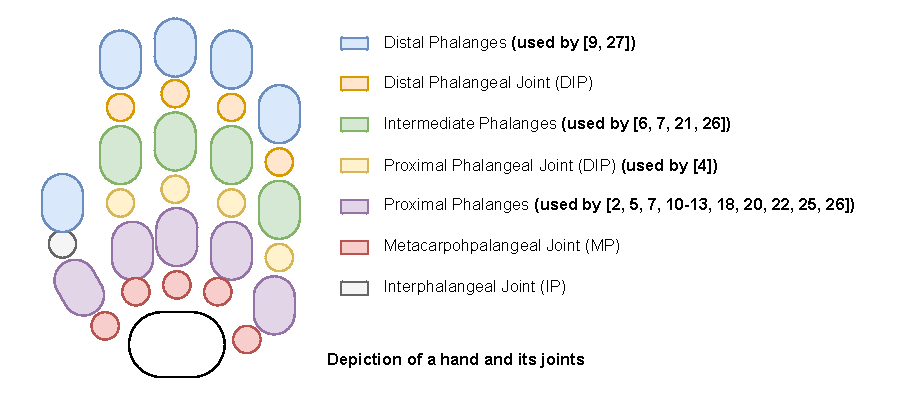
\includegraphics[width=\linewidth]{src/pictures/hand_Depiction.drawio.pdf}
    \caption{Actuator placement on the hand in previous works \cite{Learning2024,Fang2023,Fang2023a,Fang2022,Fang2022a,Donchev2021,Hsu2021,Yang2017,Seim2017,Seim2015b,Seim2014a,Seim2014, Huang2010, Vaio6810, Kohlsdorf2010, Markow2010, Huang2008}.}
    \label{fig:hand_depiction}
\end{figure}
The placement of actuators has undergone significant changes in recent research. While some studies have explored more unconventional approaches, such as the \gls{bct} used in Google Glass \cite{Seim2016a}, smartwatches \cite{Seim2018} worn on the wrist, or Velcro bands applied to the limbs for rhythm learning \cite{Bouwer2011, Holland2010}, the majority of research has focused on the skin of the hand (and occasionally the arm) as a successful site for input.
In particular, the placement of actuators on the fingers has shown that targeting the proximal phalanges is advantageous \cite{Fang2022a}, but research also explored other areas, such as the fingertips \cite{Yang2017} or even the wrist or back of the hand. \autoref{fig:hand_depiction} shows the different hand placements and their corresponding papers.
Research from Fang suggested, that the response time at the finger is shorter than for the wrist for the stimuli (vibration, taping and stroking) and the perception accuracy at the finger is significantly more accurate than at the wrist, moreover, their experimental results indicated, that the Finger Phalanx achieves higher accuracy than the Outer Wrist \cite{Fang2022a}.

\subsection{Human skin and the influences of stimulus}
\begin{figure}
    \centering
    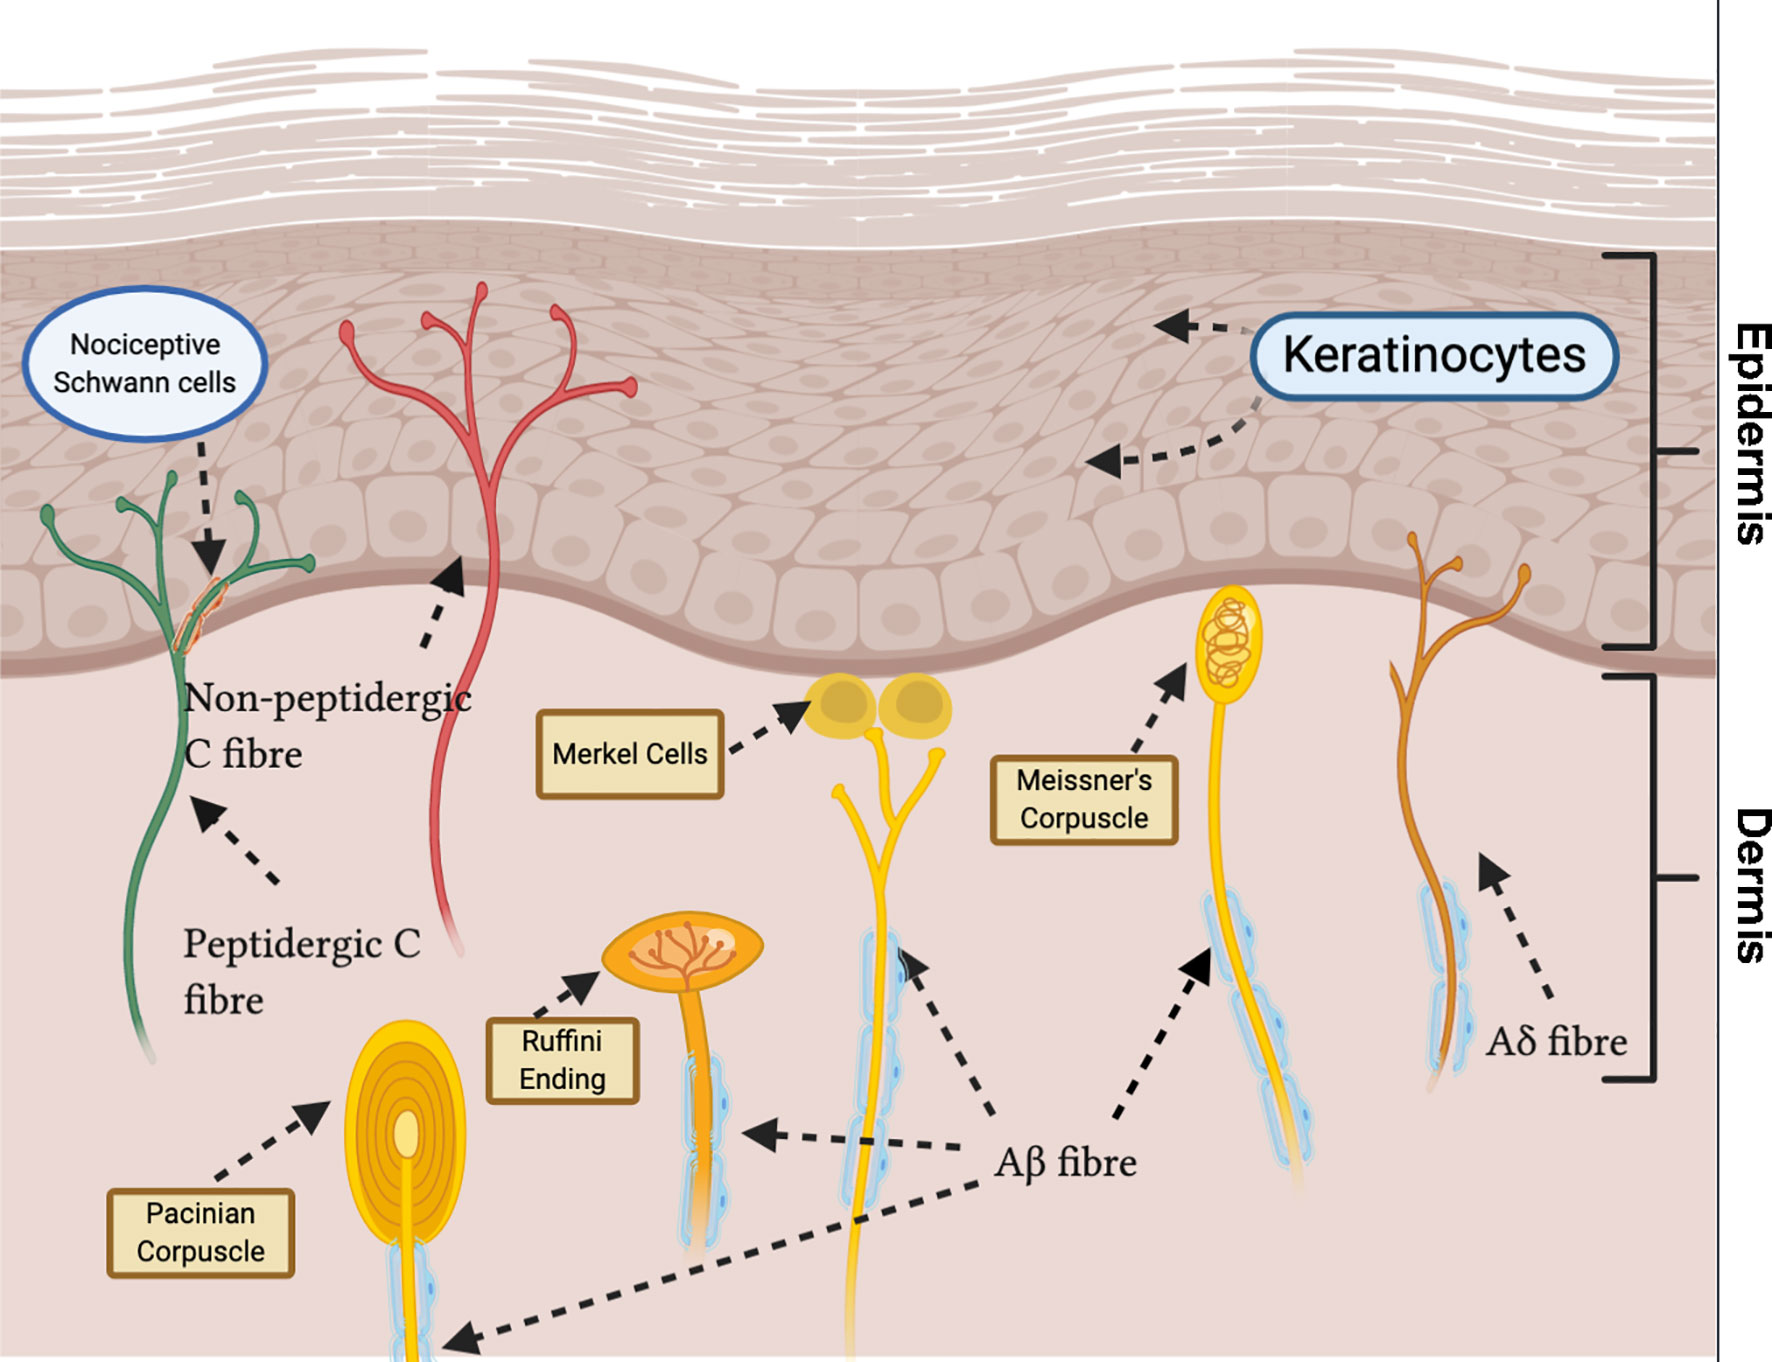
\includegraphics[width=0.7\linewidth]{src//pictures/skin.jpg}
    \caption{Depiction of the human skin \cite{lowy2021cutaneous}.}
    \label{fig:skin_image}
\end{figure}

The human skin, the largest and most visible organ of the body, serves as a versatile interface for perceiving a wide range of sensations. Beyond its protective functions, the skin provides sensory input from the environment and acts as a medium for communication and feedback. It is capable of detecting mechanical, thermal, chemical, and electrical stimuli, which generate sensations such as pressure, vibration, temperature, and pain. This diversity makes touch one of the most ancient and fundamental senses in the human body \cite{Fang2023}.

Touch perception begins at the receptors connected to nerve endings within the skin. These receptors respond to external stimuli, converting mechanical energy into nerve impulses that relay somatic sensations to the brain. Somatic sensations are those related to the physical body and include thermal, painful, and pruritic (itch-related) stimuli. The skin itself varies across the body, with glabrous (non-hairy) and hairy regions demonstrating differences in their receptor types as depicted in \autoref{fig:skin_image}, nerve fibre compositions, and the nature of the sensations they evoke. Glabrous skin, such as that on the palms and soles, is associated with discriminative touch and excels in tasks requiring precision and localization. In contrast, hairy skin regions are more attuned to affective touch and often evoke pleasant sensations, as suggested by findings in several studies \cite{Fang2023, ackerley2014quantifying,ackerley2016touch}.

Receptors in the skin fall into four major categories, collectively known as low-threshold mechanoreceptors (LTMs): Pacinian corpuscles, rapidly adapting (RA) units, slowly adapting type 1 (SA1), and slowly adapting type 2 (SA2) receptors. Each of these receptors has specialized functions, enabling the conversion of various mechanical stimuli into nerve impulses. For example, Merkel and Meissner cells detect slow pressure and low-frequency vibrations, while Pacinian corpuscles specialize in higher-frequency vibrations (up to 4000 Hz). Ruffini endings respond to skin stretching, highlighting the skin's capacity to detect spatial and temporal resolution in touch \cite{Fang2022a, Fang2023, ackerley2016touch, mcglone2014discriminative}.

These mechanoreceptors are connected to two types of nerve fibres—myelinated A$\beta$ fibres and unmyelinated C fibres—each playing distinct roles in touch perception. Myelinated A$\beta$ fibres, which are wrapped in myelin to increase signal conduction speed (20–80 m/s), project to the primary somatosensory cortex (SI area) and are primarily responsible for discriminative touch. This type of touch is crucial for localization and fine spatial resolution. On the other hand, unmyelinated C fibres, including the C-tactile (CT) afferents, have slower conduction velocities (0.5–2 m/s) and project to the posterior insula. These fibres are integral to the perception of affective touch, which is associated with emotional and social responses \cite{Fang2022a, Fang2023, ackerley2016touch, mcglone2014discriminative}.

The distinction between discriminative and affective touch is further reflected in the choice of learning devices used for passive haptic learning (\gls{phl}). The choice of device is critical to the success of \gls{phl}, as it determines the effectiveness of encoding and conveying tactile information. This study examines the impact of different haptic devices and actuator designs, differentiating between two types of input: discriminative and affective. Discriminative input encompasses sensory perceptions such as pressure, vibration, texture, or slip, whereas affective input involves motions such as sliding, tapping, and stroking \cite{Fang2023}.

Previous research has predominantly focused on vibrational input, with most studies examining discriminative input over affective input. Only a few studies have explored alternative approaches. For example, the \gls{bct} device used in Google Glass \cite{Seim2016a} is a notable example of discriminative input. In contrast, two studies specifically examined affective touch and incorporated tapping and stroking systems \cite{Fang2020, Fang2023}. These studies concluded that tapping and stroking systems are more pleasant, natural, and unobtrusive than vibrational methods for conveying information to users \cite{Fang2022a, Fang2023}. This highlights the potential of affective input methods for improving user comfort and engagement in \gls{phl}.

Past work has further explored the skin's ability to perceive stimuli through diverse actuation principles, such as vibrotactile feedback \cite{Fang2020}, skin stretching \cite{wang2019masque}, temperature modulation \cite{peiris2019thermalbracelet}, and airflow \cite{tseng2020skin}. Vibrotactile devices, for instance, use actuators to generate vibrations that are perceived by mechanoreceptors like Pacinian and Meissner cells. Low-frequency vibrations are primarily detected by Merkel and Meissner cells, while higher frequencies (up to 400 Hz) are processed by Pacinian corpuscles \cite{Fang2022a, lo1984regional}. Additionally, Ruffini cells detect skin stretching, highlighting how specific receptor types are tuned to different tactile sensations. \cite{Fang2022a, lo1984regional, Fang2022a}.

%----
\subsection*{Chorded input}


\begin{figure}
    \centering
    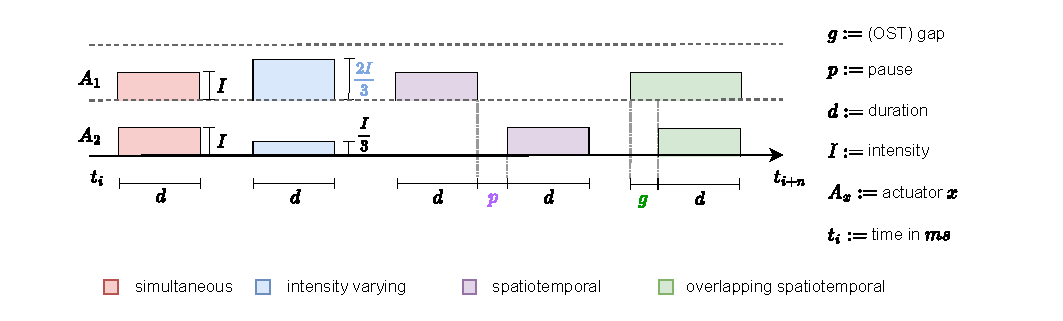
\includegraphics[width=\linewidth]{src//pictures/ost_diagram.drawio.pdf}
    \caption{Chord encoding schemes used in previous literature \cite{Luzhnica2017,Luzhnica2016,Luzhnica2018,Luzhnica2018a}.}
    \label{fig:chord_encoding}
\end{figure}

One of the primary challenges associated with Braille typing in the context of passive learning is the chorded input aspect. This refers to the simultaneous pressing of multiple keys or buttons to generate a single character, which can be particularly demanding in a passive learning environment. Chorded input often requires a high degree of motor coordination and precision, posing unique challenges for learners who lack active engagement during the learning process.

The encoding and execution of chords—actions involving the simultaneous use of multiple limbs or fingers—are central to many real-world tasks, such as playing musical instruments like the piano \cite{Seim2014, Seim2015b, Huang2008, Kohlsdorf2010, Huang2010, Seim2014a, Vaio6810, Donchev2021, Fang2023a, Fang2023}, performing multi-limb rhythms on drums \cite{Bouwer2011, Holland2010}, and Braille writing itself \cite{Learning2024, Seim2017, Seim2014a}. These activities demand the integration of complex motor skills, making them particularly challenging to teach through passive learning. As such, developing effective methods to teach users how to perform chords is crucial.

Several approaches have been explored to encode and teach chorded inputs, as illustrated in Fig. \autoref{fig:chord_encoding}. Seim et al. identified that encoding chords is especially challenging due to the difficulty participants face in accurately distinguishing simultaneous stimuli of multiple fingers, a problem depicted in red in Fig. \autoref{fig:chord_encoding} \cite{Seim2014, Seim2015}. 

In an attempt to address these challenges, Luzhnica et al. investigated the use of varying stimulus intensities (depicted in blue in Fig. \autoref{fig:chord_encoding}) to differentiate between inputs. However, this approach proved to be ineffective, as the variation in intensity did not provide sufficient clarity for learners to distinguish between stimuli \cite{Luzhnica2017}.

A more promising method, proposed by Seim et al., involves staggered input, where stimuli are activated or deactivated sequentially rather than simultaneously (depicted in purple in Fig. \autoref{fig:chord_encoding}). This spatiotemporal encoding method, first introduced by Seim et al. \cite{Seim2014a} and adopted in subsequent studies \cite{Seim2014}, enables a clearer temporal distinction between stimuli. By presenting stimuli sequentially, learners are better able to recognize and understand chord patterns, improving learning outcomes. However, this approach has limitations, particularly with encoding speed. The sequential nature of the method can slow down the process, especially for complex chords, thereby impacting overall learning efficiency.

To overcome these speed limitations, Luzhnica et al. introduced the \gls{ost} encoding method, depicted in green in Fig. \autoref{fig:chord_encoding}. This method improves upon the spatiotemporal approach by overlapping the activation of actuators. Specifically, one actuator is turned on, followed by a delay (the OST-gap $g$) before activating the next, with all actuators remaining active for a fixed duration $d$ before being turned off simultaneously. The \gls{ost} method not only enhances encoding speed but also ensures that patterns are maintained longer, improving both accuracy and the overall learning experience \cite{Luzhnica2018, Luzhnica2018a, Luzhnica2017, Luzhnica2016}.

Further refinements to the \gls{ost} encoding method were explored in a follow-up study by Luzhnica et al. \cite{Luzhnica2017}. They found that prioritizing more sensitive areas of the skin during the \gls{ost} encoding process improved accuracy while increasing the delay between activations had little impact on performance. These findings highlight the robustness and effectiveness of the \gls{ost} method in addressing the challenges of chorded input in passive learning \cite{Luzhnica2017}.


\section{Braille Learning}
\begin{figure}
    \centering
    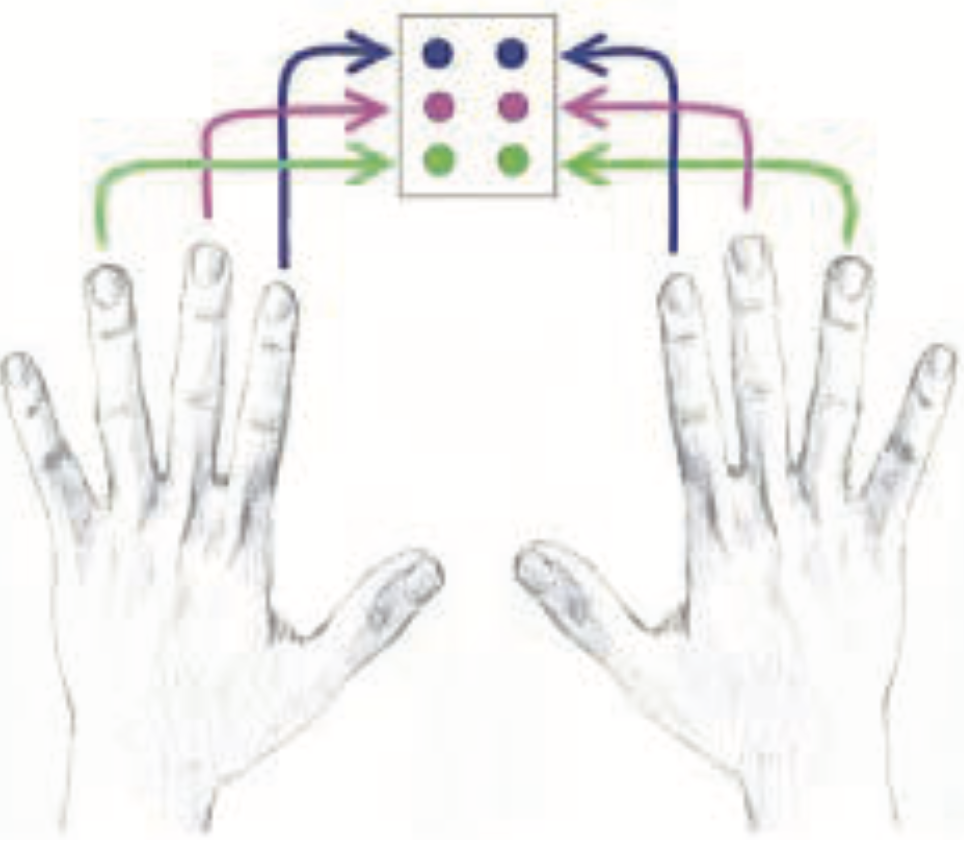
\includegraphics[width=0.5\linewidth]{src//pictures/Screenshot 2024-09-12 at 20.13.38.png}
    \caption{Braille finger mapping \cite{Seim2014a}.}
    \label{fig:braille-key-mapping}
\end{figure}
\begin{figure}
    \centering
    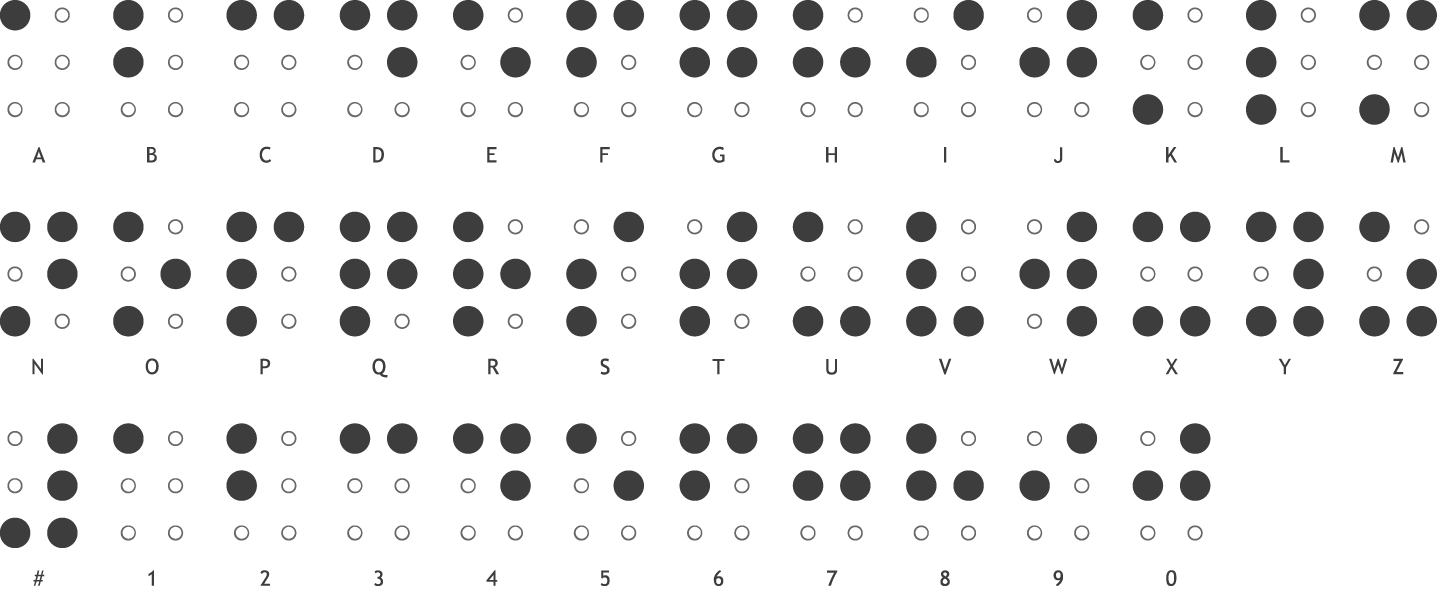
\includegraphics[width=0.5\linewidth]{src//pictures/braille_alphabet.png}
    \caption{English Braille alphabet (Grade One) \cite{pharmabrailleBrailleAlphabet,troughton1992guidelines}.}
    \label{fig:braille-alphabet}
\end{figure}
Braille, a tactile writing system, was developed in 1825 by Louis Braille\footnote{\url{https://www.dbsv.org/wie-die-brailleschrift-funktioniert.html}}. It is composed of a six-dot system, as illustrated in Fig. \autoref{fig:braille-alphabet}, which allows users to type characters by pressing combinations of six keys simultaneously, as shown in Fig. \autoref{fig:braille-key-mapping}. Devices like the Perkins Brailler, the most commonly used Braille typewriter, facilitate this process. The Perkins Brailler consists of six main keys for typing, along with a space bar and secondary keys \cite{Wikipedia2023}. Despite its utility, teaching and learning Braille remains one of the most significant challenges, particularly due to the time-intensive nature of mastering the system.

The integration of technology in Braille education has gained traction but remains underutilized, especially for senior learners. A 2018 study by Martiniello et al. \cite{Martiniello2018} found that while 62.5\% of \gls{tvi} and Rehabilitation Specialists working with younger learners use technology in their instruction, only 26.3\% do so with seniors. Rehabilitation Specialists were also found to use technology less frequently than \gls{tvi}, though \gls{tvi} reported that technological tools enhance learner motivation and improve outcomes. Among these tools, the Braille Tutor app stands out. Available on multiple platforms, it has been downloaded over 100,000\footnote{\url{https://play.google.com/store/apps/details?id=com.lukeneedham.brailletutor&hl=en}\\and \url{https://brailliac.com/}} times. McCarthy et al. \cite{McCarthy2016} demonstrated that the app increased students’ learning rates, allowing them to achieve 100\% accuracy faster and learn more Braille contractions—a shortened form of Braille words, also called Grade two Braille\cite{troughton1992guidelines}.

In addition to digital methods, non-digital programs such as the Mangold Braille Program \cite{Mangoldnd} and resources from Hadley\footnote{\url{https://hadleyhelps.org/learn?topic_id=15}} play a vital role.
The Mangold Program focuses on tactile perception and symbol recognition before introducing the Braille alphabet through 29 progressive lessons. Hadley, endorsed by the New York State Commission for the Blind (NYSCB)\footnote{https://ocfs.ny.gov/programs/nyscb/assets/docs/BrailleFAQ.pdf}, offers self-learning resources but emphasizes that learning Braille, particularly contracted Braille, is a lengthy process, often requiring over a year. Tools like Alpha Boxes\footnote{https://www.pathstoliteracy.org/alpha-boxes/}, which pair initial letter sounds with Braille symbols, provide additional support for early learners.

Despite these resources, one-to-one teaching between students and teachers remains the dominant method for Braille instruction, as noted by Jawasreh et al. \cite{Jawasreh2020}, who developed the Braille Finger Puller, a haptic device aimed at innovating the teaching process. Similarly, haptic technologies, such as the Translation Glove by Subathra et al. \cite{Subathra2024}, have been designed to use vibrations to support Braille learning, akin to the gloves developed by Bandodkar et al. \cite{Bandodkar2014} and Shivakumarl et al. \cite{Shivakumarl2013}. However, most devices rely on vibration gloves, with few exploring \gls{phl}. Like Seim et al. and Caulfield et al., \cite{Learning2024} have investigated this technique, though it remains underutilized in existing Braille learning devices. Furthermore, none of the current technologies incorporate \gls{ost} encoding, a method with significant potential to improve tactile learning efficiency.

Studies have also explored Braille learning among sighted individuals. Bola et al. \cite{Bola2016} conducted a nine-month study with 29 sighted adults, mostly Braille teachers, and found that participants could read Braille at an average speed of six words per minute by the course’s end. Interestingly, low tactile accuracy did not significantly affect reading speed, indicating that even sighted individuals can adapt their sensorimotor systems to Braille without visual deprivation. Their learning rate was comparable to congenitally or early blind children learning Braille in primary school. Some educators have even employed methods like blindfolding children with residual vision to accelerate their tactile learning \cite{Bola2016}.

Additional research has focused on variables influencing Braille learning rates. Hall et al. \cite{Hall1987} identified study modality (visual or haptic), stimulus discriminability, and test modality as key factors affecting performance during the learning phase. These insights have informed the development of teaching strategies and tools to better accommodate diverse learners.

Despite advancements, learning Braille remains a slow and challenging process, often requiring months or even years to achieve proficiency, particularly in contracted Braille. This underscores the need for further innovation in teaching methods and devices, particularly those incorporating \gls{phl} and \gls{ost} encoding, to enhance the efficiency and accessibility of Braille instruction.




